\documentclass[a4paper,12pt]{book}
\usepackage{listings}
\usepackage{color}

\definecolor{dkgreen}{rgb}{0,0.6,0}
\definecolor{gray}{rgb}{0.5,0.5,0.5}
\definecolor{mauve}{rgb}{0.58,0,0.82}

\lstset{frame=tb,
  language=Java,
  aboveskip=3mm,
  belowskip=3mm,
  showstringspaces=false,
  columns=flexible,
  basicstyle={\small\ttfamily},
  numbers=none,
  numberstyle=\tiny\color{gray},
  keywordstyle=\color{blue},
  commentstyle=\color{dkgreen},
  stringstyle=\color{mauve},
  breaklines=true,
  breakatwhitespace=true,
  tabsize=3
}


\usepackage{times,a4wide}
\usepackage{graphicx}
\usepackage{amssymb}
\usepackage{epstopdf}
\DeclareGraphicsRule{.tif}{png}{.png}{`convert #1 `dirname #1`/`basename #1 .tif`.png}
\usepackage[round]{natbib}
\usepackage{html}
\title{Procedural Terrain Generation for Games}
\author{Fabio Peres Filho\\ma301fp\\ \\Supervisor: Professor Dr Marco gillies}
\date{\today}                                           % Activate to display a given date or no date

\begin{document}
\maketitle
\def\thepage{\roman{page}}
\part{The Report}
\chapter*{Abstract}
Procedural Terrain Generation for Games is a project that aims to create procedurally, a height map using random numbers generator and perlin noise, generate maps, display them and create mesh out of them using the related mathematical techniques, Unity3D game engine and Visual Studio as text editor. 

\newpage

\chapter*{Acknowledgements}
I would like to thank everyone who was involved in this project somehow, in particular I would like to thank Marco Gillies for spending his time supervising me in this project and for his guidance and advice through the course and this project. I also need to give a big thank you to Lahcen Quarbya and Kate Devlin, for supporting me when times were pretty dark in my life. A special thank you for Liam Robinson, my classmate and currently business partner for helping always push a little more when coding come to the table, another one to Aonghus O’Kelly, good friend and adviser.
A huge thank you to my family, my father Miguel Peres Filho, my mother Magda Freire Peres and my brother, Rodrigo Freire Peres for always believe on me and to my dear wife Krittika Phakbunduphong, for all support along last three years. 


\tableofcontents
\listoffigures
\listoftables

\chapter{Introduction}
\def\thepage{\arabic{page}}
\setcounter{page}{1}

\section{The Project and Aims}


This project is named Procedural Terrain Generation Project and as the name suggests it will use procedural content generation - PCG – and related techniques, a good understanding of random numbers generation, such as noise, and triangles to create meshes. The aim here is to produce terrain meshes and different biomes using height map to produce random numbers. 


%\newpage
\section{Motivation}

The idea for this project came after I gave up a super ambitious idea to make a MMO for this project. As my supervisor Marco advise me that would be too much to research and implement for the time available for doing this project. 
Then after looking on the internet about old games styles with friends, the game ‘Diablo I’ came to my screen. I was always intrigued by the fact that every time I played this game, all dungeons were different. Besides any boss level, all level maps were different. After some very preliminary research about those maps, I have discovered that the maps were actually created procedurally and not architecture by an artist level designer of some kind. 
Allied to the fact that I was extremely involved in a level design map in a project during my second year, ‘The Midnight Man’ project, it seems to be irresistible the possibility to create a level map again but at this time with a different approach, instead of doing a terrain map using a  graphical 3D renderer software to create the level, I could use procedural content generation to create the map using just code, what would be a perfect project idea taking in mind that my degree is a programming oriented course.


\section{Required Tools}

The project will be produced by using the Unity3D game engine, and such requires a very good understanding of C-sharp programming language. In addition to that, mathematical understanding of random numbers generation, in particularly to noise and perlin noise to produce a height map that will be used to determine the shape of the terrain level. Once the shape of the terrain is done, we will  generate meshes based in a colour map and set the height of the Y-axis to the height value generate by the noise function.
 

\section{The layout of my report}

In Chapter~\ref{chap:backgroundResearch}, I discuss and demonstrated almost all the research done about random number generator, noise, perlin noise, procedural content generation definitions, applicability and relevance to this project 

In Chapter~\ref{chap:systemDesign},I design how to and determine how the system is build.

In Chapter~\ref{chap:implementation},I explain how the the main features of the code works and why they are design in the way that they were.


\chapter{Background Research}
\label{chap:backgroundResearch}

This chapter will list and detail most of the research undertaken for this project, but not all, since before starting the development of the project itself, during the development and further research on later stages of the implementation. I would say the research for this project could defined as a ‘work in progress research’. 

\section{Procedural Content Generation Definition}
\label{sec:PCGD}

Before start the overview of procedural content generation and defines what it is, we need to start with something a little bit more dry: definitions, of course. 
Julian Togelius on his book, ‘What is Procedural Content Generation?’ (2011) stated the definition of procedural content generation as the algorithmical creation of content with limited or indirect user input.
That means, PCG is related to a software that can create own its own, or using parameters entered in the system by a user, content.
  


\subsection{Definition of the word Content}
\label{sub:DOTWC}

The definition of content here is my own definition after extensive research. Content here is anything that can be described and coded. If you can describe a feature, what it is, how it works or how it could behave, then a programmer can code this feature. Content here is this feature. Could be many things, such as terrains, levels, maps, textures, items, music. Bringing this more related to games (after all I am a game programming student), content could easily be quests, weapons, cars, cities, enemies, world maps, set of rules that must be follow by an AI agent (such as in Stellaris).
Therefore, the word content here cannot be misunderstood as the game itself or a non-player character behaviour – NPC. The game itself is not considered to be content itself because it is not created completely by a software although it is a software. A Non player character behaviour is a method related to artificial intelligence – AI -  as an autonomous agent instead of procedural content. PCG is of course a branch of artificial intelligence, because it is largely based on AI methods.


\subsection{Definition of Procedural and Generation}
\label{sub:DOPAG}

The word generation is almost self-explanatory, is means something created by the procedural method of generation (creation). Procedural is related to something created by procedures. A computer follows procedures to executes code. Therefore, procedural is an algorithm, is computer code that creates, generates something (content).


\subsection{Procedural Content Generation in Games}
\label{sub:PCGIG}

Procedural content generation in games is when part of the game, some features or just one of its features are created and generated by code, without data entered by the user or with indirect input by the gamer/user.
These features could be of many types and for many different reasons. For example:

In the game series Diablo, created and developed by Blizzard Entertainment Inc., there is a PCG feature that creates dungeons for an action, role play game – RPG, hack-and-slash game without any input by the player-hero.

In the game series Civilization, Sid Meyers Studios uses procedural content generation to create the world map, without user input or with few parameters input by the user, such as size of the world, type of the world (which includes temperature of the world, age of the world, level of water of the world). All those parameters changes how the final world map will look like, but the landscape and shape have no parameters what so ever.

PCG could be used to populate a world with vegetation, animals, people, etc.

A feature that procedurally generates different races with different traits in every single game in Stellaris.

And of course, a feature that could generate a terrain map, with or without different biomes for a game as well, which is the scope of this project.


\subsection{Why use PCG and Existing Games Using PCG}
\label{sub:WUPAEGUP}

Nowadays, exists almost an uncountable number of game studios that uses procedural content generation as a tool to create part of the features of their games.
One of the first and maybe most important reason to procedurally create game content is financial. Human work is either expensive and slow (comparing to computers for calculations). If one can remove the human component (an artist or level game designer) for example, and replace it with a creating of content by code, that means, procedurally generation, it reduces the costs significantly, which gives more room to a game become profitable and then commercially successful. 
Another reason is the fact that, to procedurally create something, the description must be near perfection.  If one can describe so good a system, this person will understand better the design process of that feature, which increases the performance of the system that uses it.
For one of the two reasons above, or even for another reason not actually mentioned on this report, some of the listed games below incorporated procedural content generation of some kind on their games:

\begin{figure}
\begin{center}
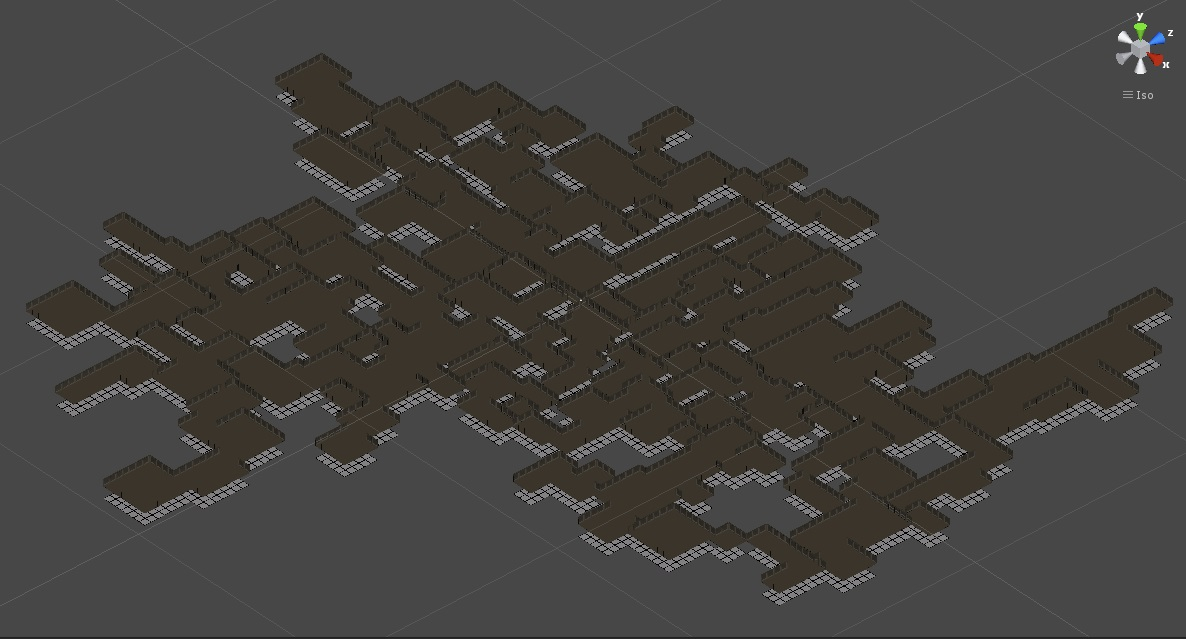
\includegraphics[height=70mm]{diablo_series_1.jpg}
\end{center}
\caption{Screen-shot of a dungeon map in Diablo series}
\label{fig:2.1}
\end{figure}

\begin{figure}
\begin{center}
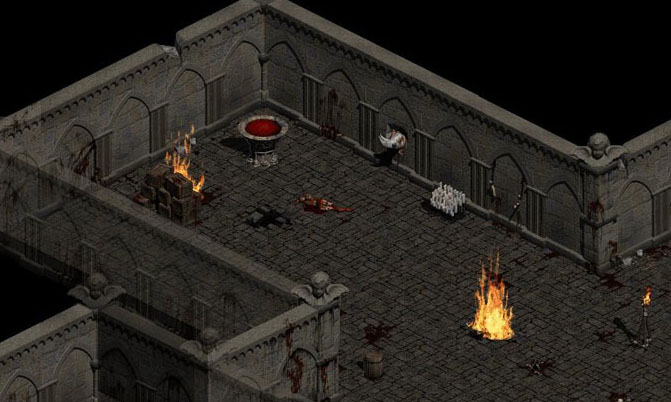
\includegraphics[height=70mm]{diablo_series_2.jpg}
\end{center}
\caption{Screen-shot of a dungeon in Diablo series}
\label{fig:2.2}
\end{figure}

Map terrain generated in the Civilization series:

\begin{figure}
\begin{center}
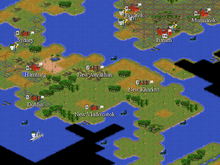
\includegraphics[height=70mm]{civ-series.png}
\end{center}
\caption{Screenshot of a terrain map in Civilization II}
\label{fig:2.3}
\end{figure}

Another example of game using terrain generation is Minecraft

\begin{figure}
\begin{center}
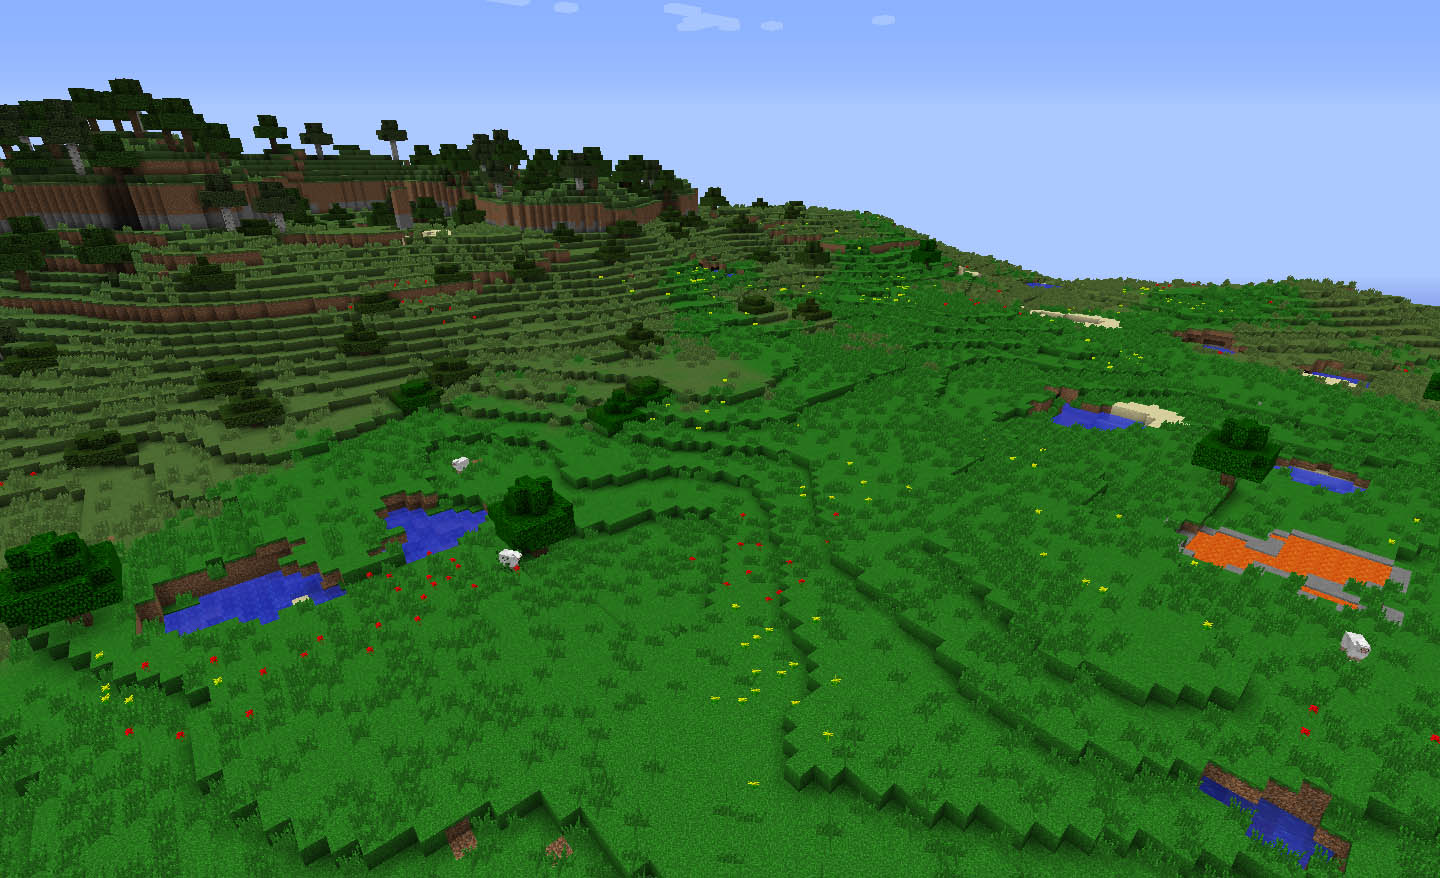
\includegraphics[height=70mm]{minecraft.jpg}
\end{center}
\caption{Screenshot of a terrain map in Minecraft}
\label{fig:2.4}
\end{figure}

\section{Random Numbers Generation and Seed}

There are two main methods today to generate random numbers. The first method of generate random numbers is to measure physical phenomena. These physical phenomena are expected to be random. Example of this is atmospheric noise, thermal noise and quantum phenomena. 
The second type of random numbers generation is the one that actually interest to this project, the computational algorithms that can produce very long streams of apparently random results. This sequence of random numbers, are in fact completely determined by a shorter initial value know as seed value or key.
As a product of this seed or key, the entire result that seems to be a random sequence of numbers, can be reproduced any time on demand, if and only if the exact same seed is entered again in the algorithm that generates the random number, reason why is also called pseudo-random numbers.
In conclusion, a pseudo-random number generator based only on a deterministic logic (not include natural source), can never be considered as a “true” random number. The function that actually calculate this number will eventually show some form of pattern, but the time consumed to us notice that is so big, that we still can use as ‘randomness’.
There are also some other methods that try to generate a random number based on a probability density function, or generation from a probability distribution.


\subsection{Probability and Non-Uniform Distribution}

Probability is defined in the Wikipedia as the measure of the likelihood that an event will occur. Probability is scale from 0 to 1, where 0 is the impossibility and 1 is the certain occurrence of the event.
A non-uniform distribution is when some weight is added to the probability of an event. For example: if a random number generator is set to return 3 values, 1, 2 or 3. If we add those numbers to an array of size 5, and add number 1 to first two elements of the array, number 2 to the third element and number 3 to fourth and fifth elements, then we randomly generate a number between 1 and 5, which will return on of the elements of the array, we have a non-uniform distribution of the numbers 1, 2 and 3, because we have 40 percent chance to return number 1 and 3 and 20 percent to return number 2.

\subsection{Normal Distribution of Random Numbers}

Normal distribution, also known as Gaussian Distribution is when all values are in a determined range but they are clustered at the average or mean point between both minimum and maximum values.
Any value is generated by a function, which is defines the probability of likelihood that value can occur, comparing it to the mean.
In a Gaussian Distribution, some concepts are important to define: mean, difference from mean, variance, average variance and standard deviation.
The mean is calculated by the average of the values. 
Difference from mean is the subtraction of the value by the mean, on this order.
Variance is square root of the difference from mean of the value previously calculated by difference from mean.
Average variance is the average of all variance values, added together and divided by the number of values.
Standard deviation is the square root of the average variance.
The following example was extracted from Daniel Shiffman, “The Nature of Code”, 2012, online version at http://natureofcode.com/book/introduction/ last visited on 15/08/2016.

\begin{figure}
\begin{center}
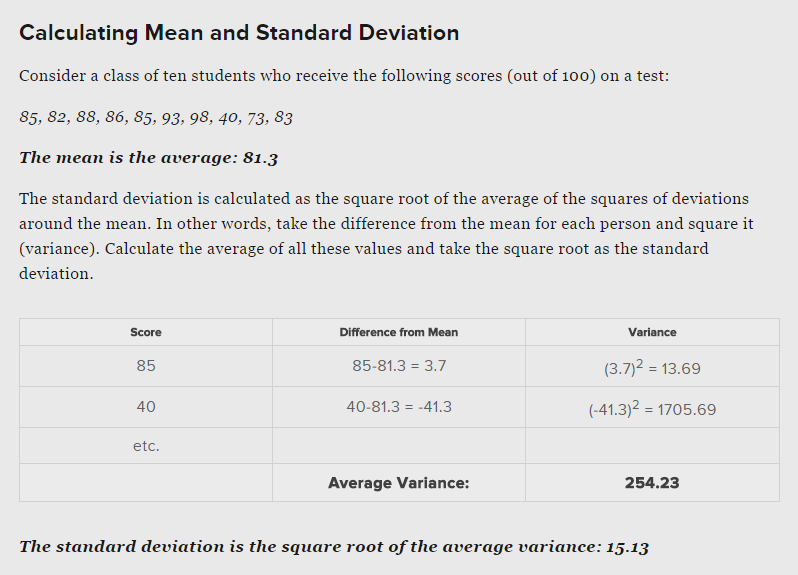
\includegraphics[height=90mm]{normal_distribution-chart.png}
\end{center}
\caption{How to calculate Mean and Standard Deviation}
\label{fig:2.5}
\end{figure}

\subsection{Perlin Noise}

Perlin Noise is an algorithm that is used often in procedural content generation. It is especially useful for games and was invented by Ken Perlin.
The algorithm is a type of gradient noise.

\begin{figure}
\begin{center}
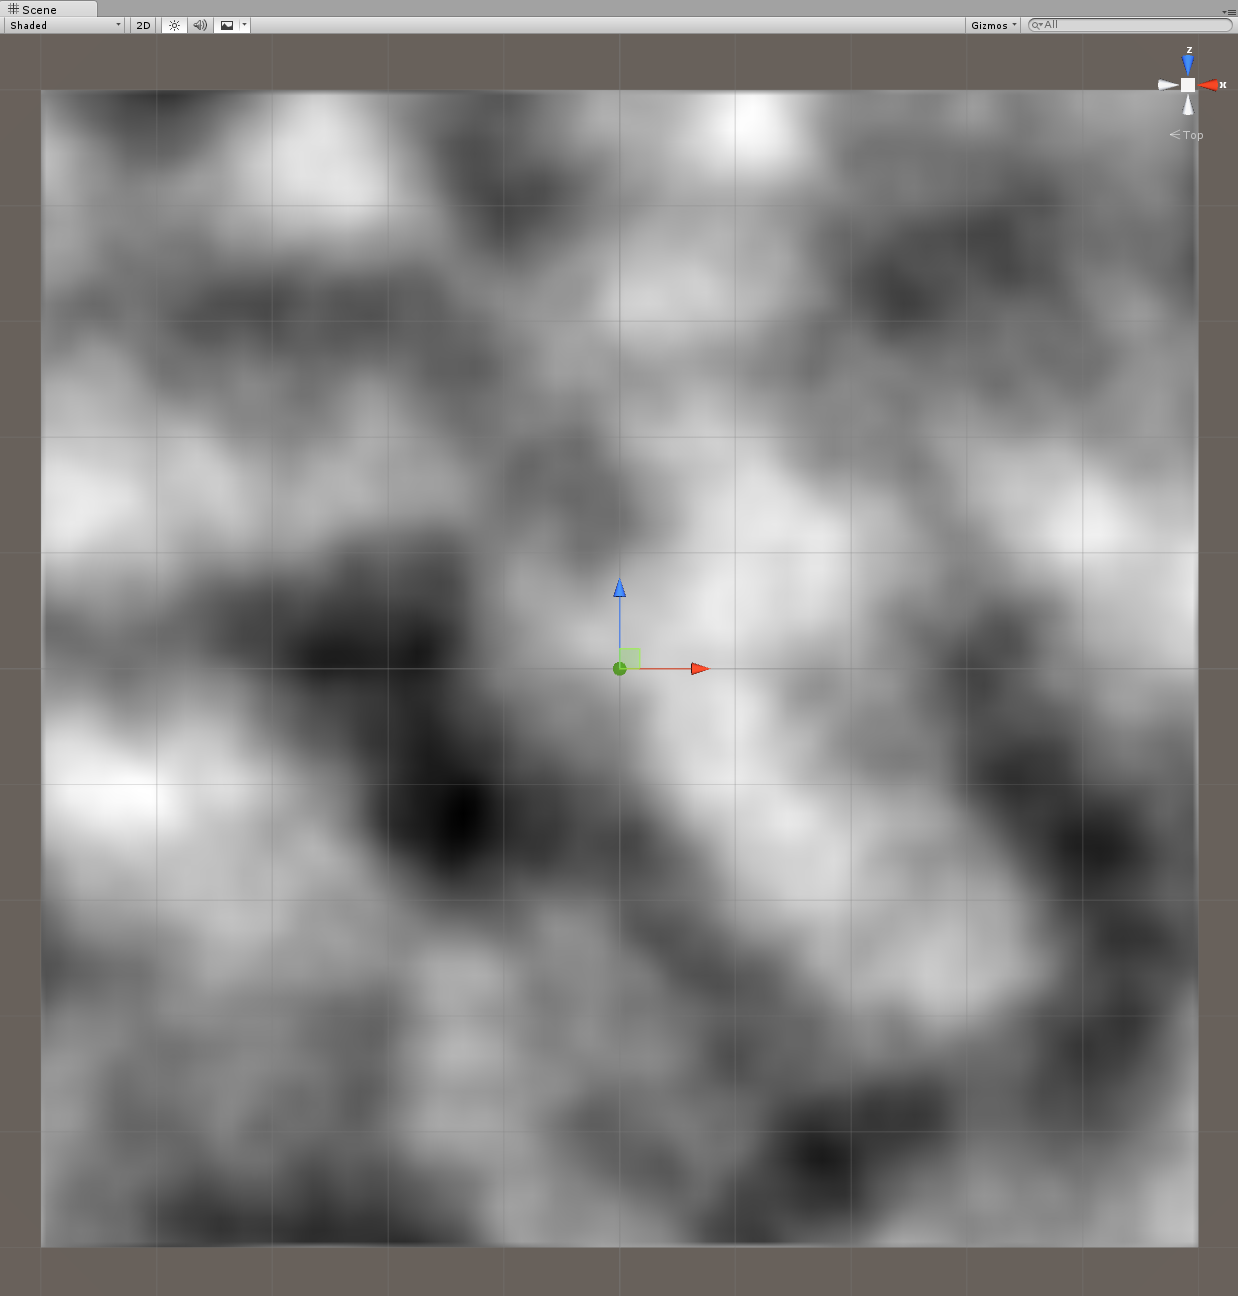
\includegraphics[height=80mm]{Detailed_Map_Noise_Example.png}
\end{center}
\caption{Two-dimensional slice of perlin noise gradient extract from the code}
\label{fig:perlinNoise}
\end{figure}

Perlin noise is a procedural texture primitive and is very good to increase realism and smoothness in computer graphics.

The algorithm itself is divided in three main parts: Grid Definition, Dot Product and Interpolation.

Grid Definition define an n-dimension grid. The variable n is commonly used as a two, three or four dimensions.

The dot Product part of the algorithm is related to given a n-dimension argument for the noise function the algorithm will determine where a point will fall in a specific part of the grid

The final step is interpolation between the ${\displaystyle 2^{n}}$dot products computed at the nodes of the cell containing the argument point. This has the consequence that the noise function returns 0 when evaluated at the grid nodes themselves (definition extract from a online source at \cite(Perlin, Ken (July 1985). "An Image Synthesizer". SIGGRAPH Comput. Graph. 19 (0097-8930): 287––296. doi:10.1145/325165.325247. Retrieved 9 February 2016.)

\begin{figure}
\begin{center}
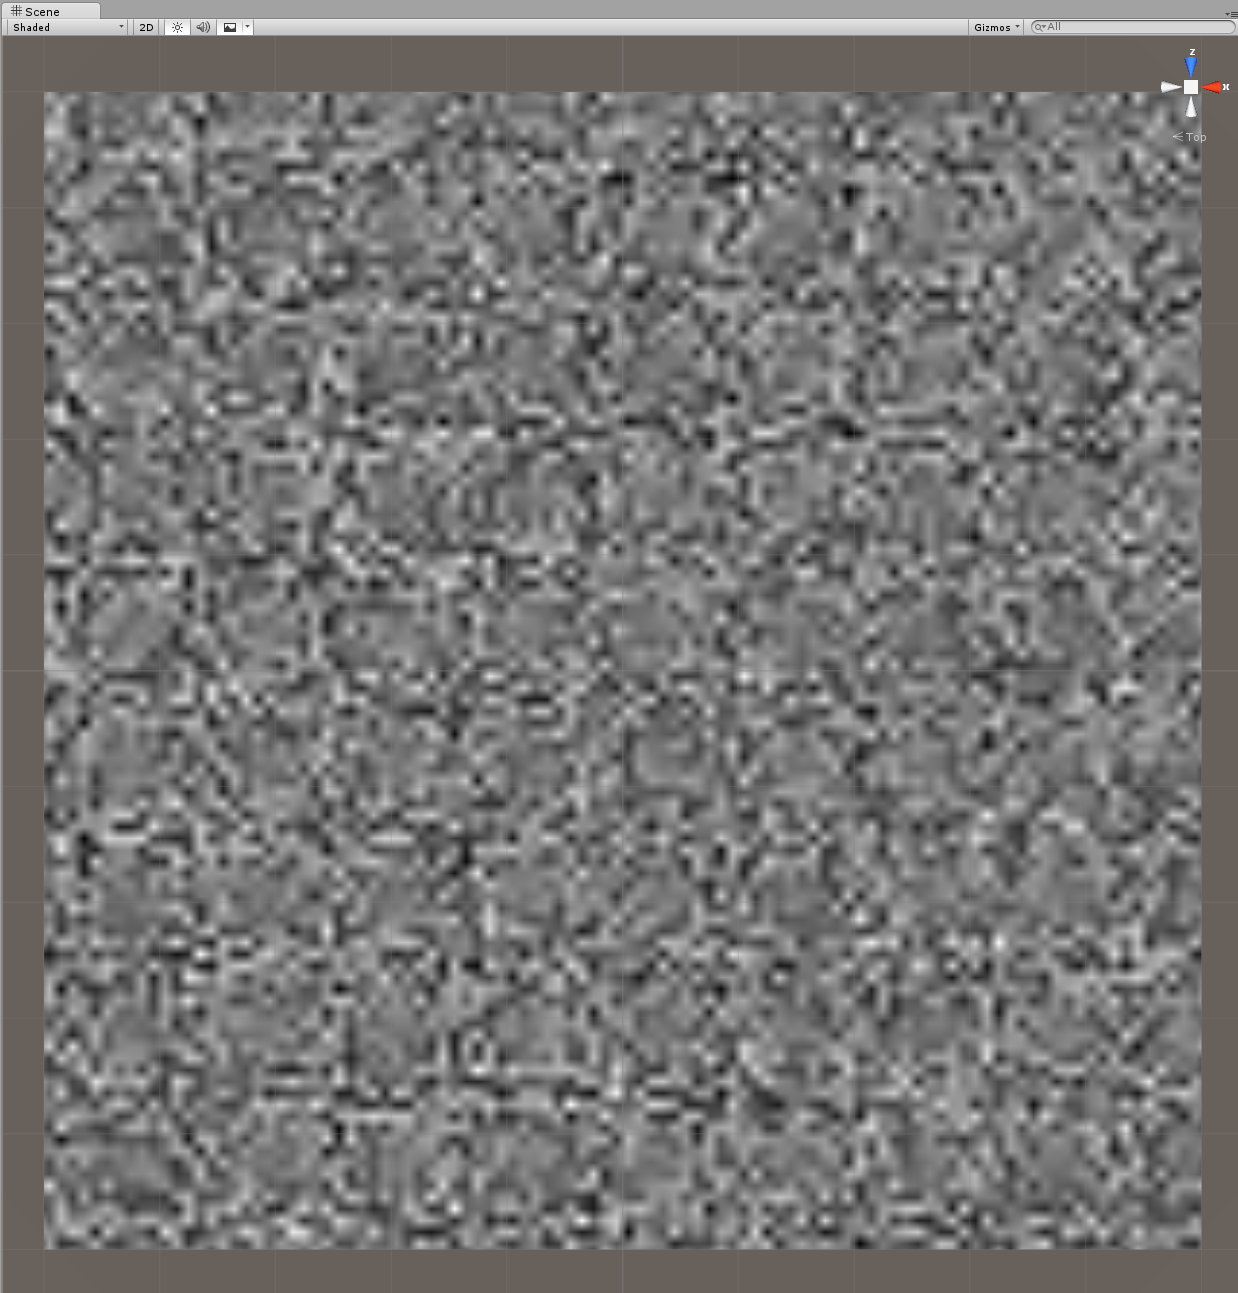
\includegraphics[height=80mm]{Map_Noise_Example.png}
\end{center}
\caption{Regular noise}
\label{fig:pretty}
\end{figure}


\chapter{System Design}
\label{chap:systemDesign}

This chapter describes superficially the system design process to the success of the project and to be able to achieve its aims.

\section{Terminology}


Amplitude is related to the Y-axis

Frequency is related to the X-axis

An octave is consisted of a noise map

Number of octaves is related to the number of layers of noise map

Lacunarity control the increase in frequency of octaves

Persistance control the decrease in amplitude of octaves



\section{How Amplitude, Frequency, Lacunarity and Persistance works}


\begin{figure}
\begin{center}
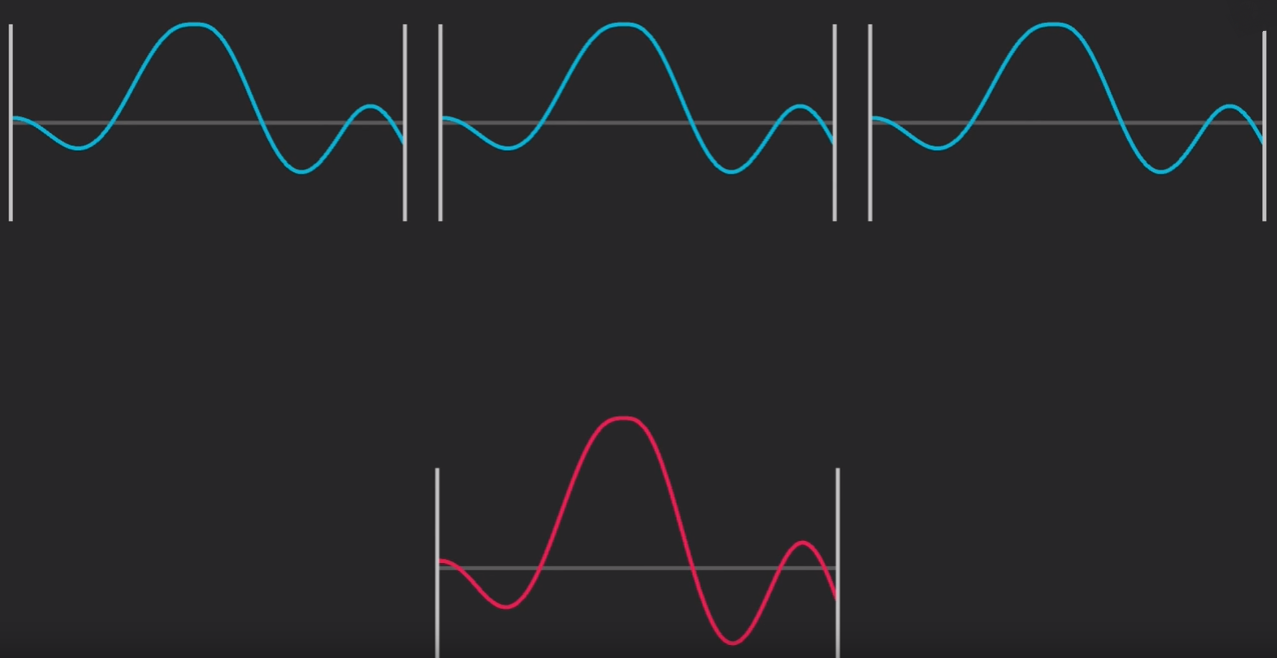
\includegraphics[height=80mm]{3noise-maps-octaves.png}
\end{center}
\caption{3 octaves waves, Y-axis is amplitude and X-axis is frequency}
\label{fig:pretty}
\end{figure}

\begin{figure}
\begin{center}
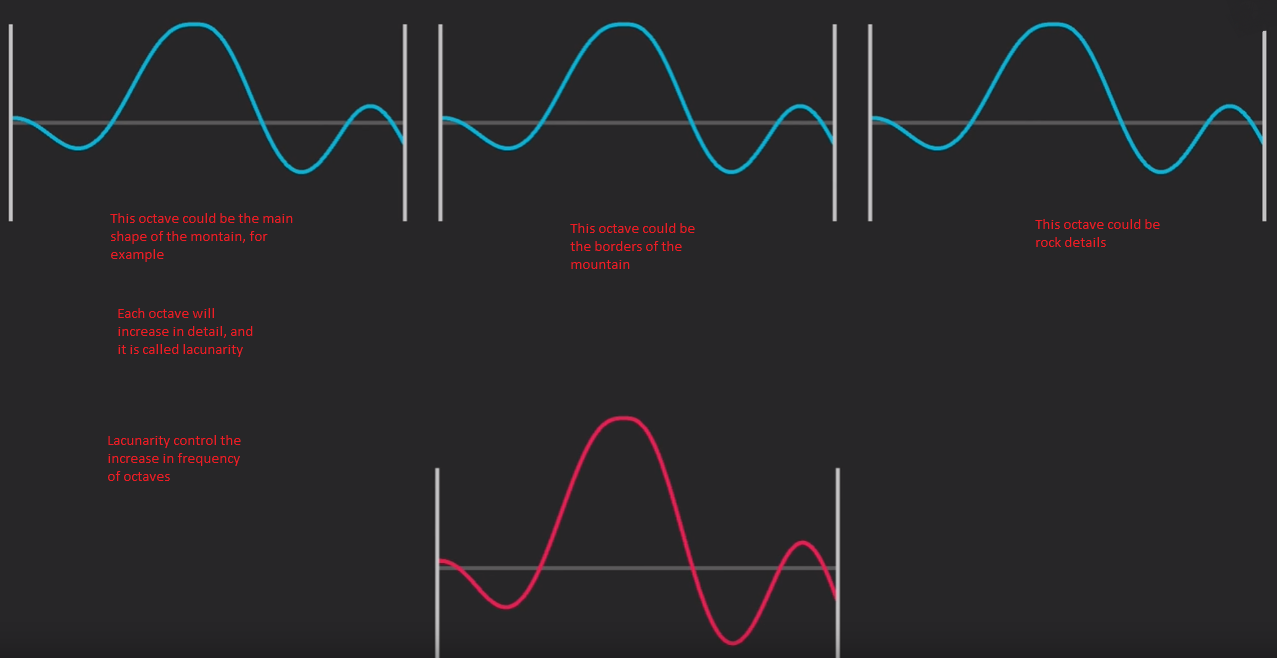
\includegraphics[height=80mm]{3noise-maps-octaves-2.png}
\end{center}
\caption{3 octaves waves, Y-axis is amplitude and X-axis is frequency}
\label{fig:pretty}
\end{figure}

\begin{figure}
\begin{center}
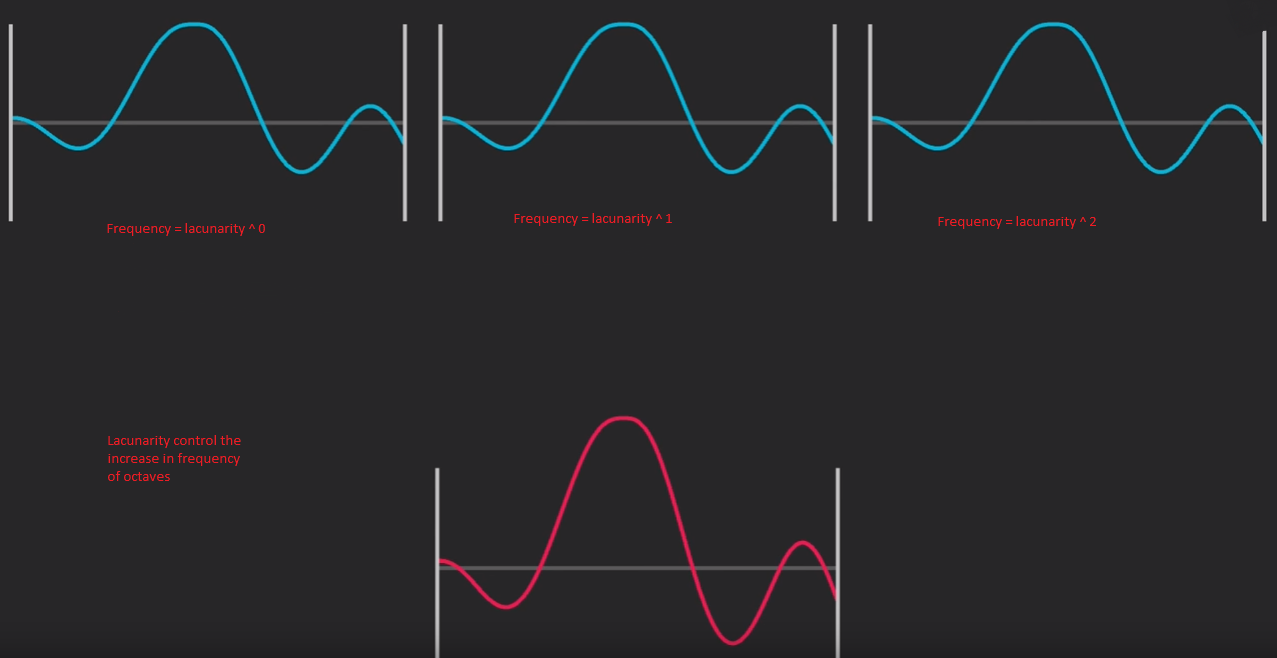
\includegraphics[height=80mm]{3noise-maps-octaves-3.png}
\end{center}
\caption{3 octaves waves, Y-axis is amplitude and X-axis is frequency}
\label{fig:pretty}
\end{figure}

\begin{figure}
\begin{center}
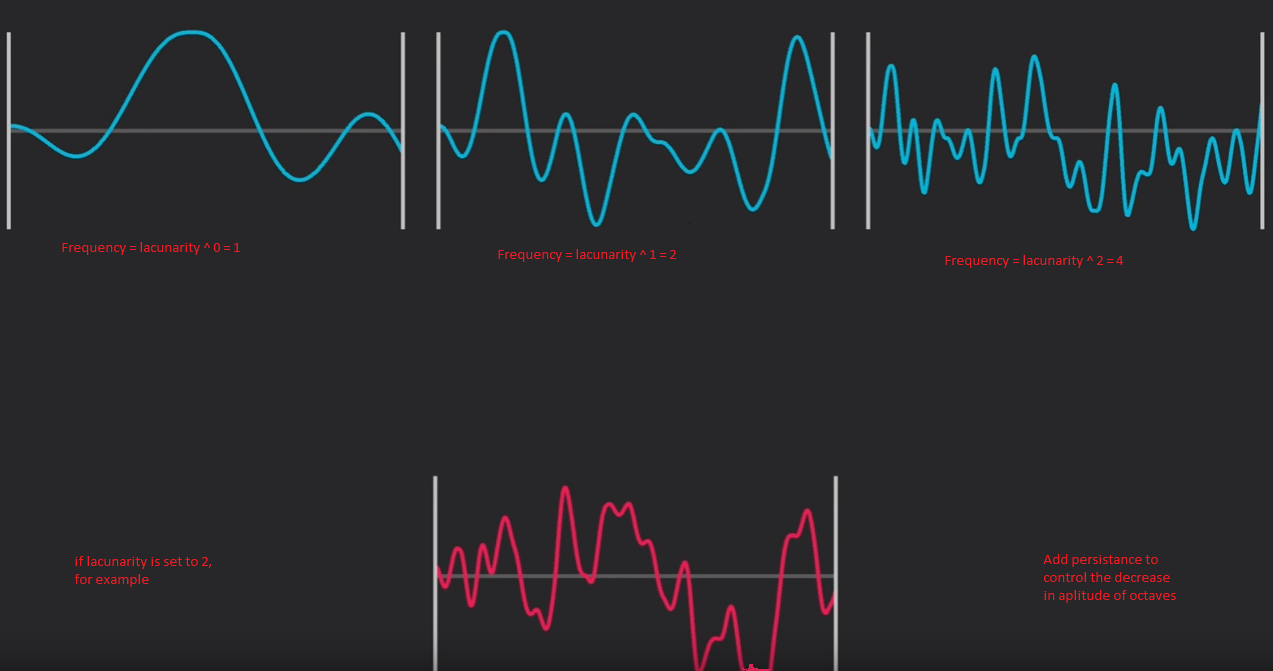
\includegraphics[height=80mm]{3noise-maps-octaves-4.png}
\end{center}
\caption{Lacunarity is applied to control the increase in frequency}
\label{fig:pretty}
\end{figure}

\begin{figure}
\begin{center}
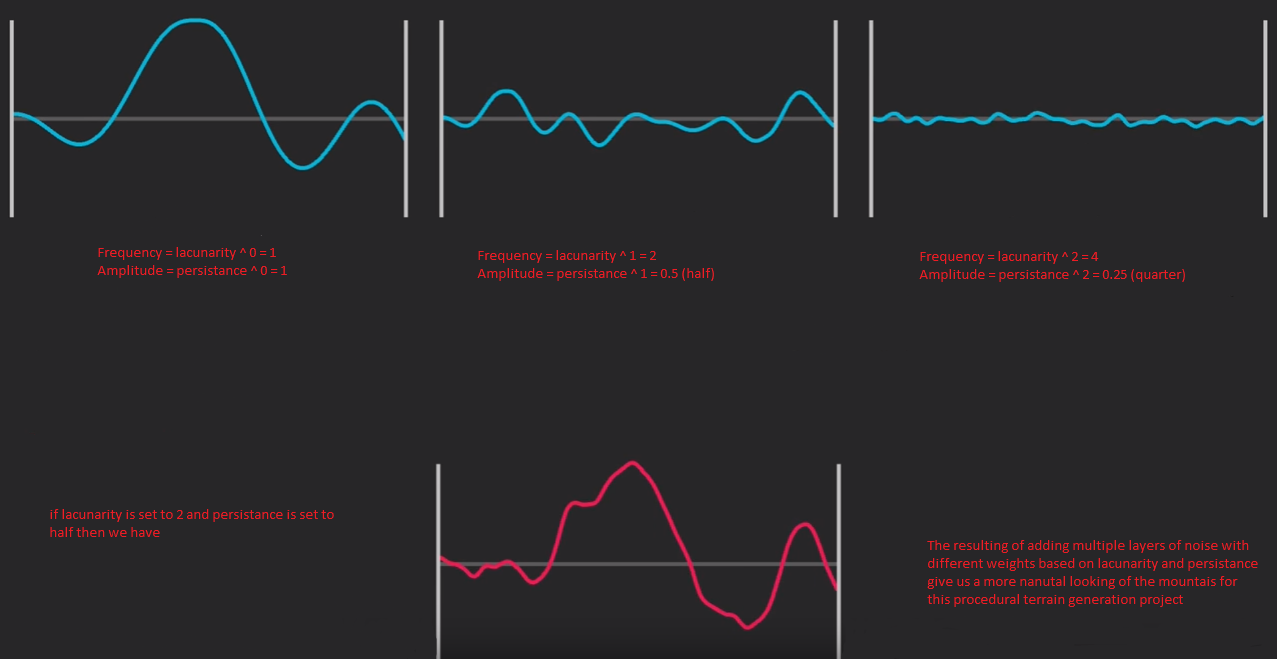
\includegraphics[height=80mm]{3noise-maps-octaves-5.png}
\end{center}
\caption{Persistance is applied to control the decrease in amplitude}
\label{fig:pretty}
\end{figure}


\section{How the Triangles are Calculated to Create the Mesh}

\begin{figure}
\begin{center}
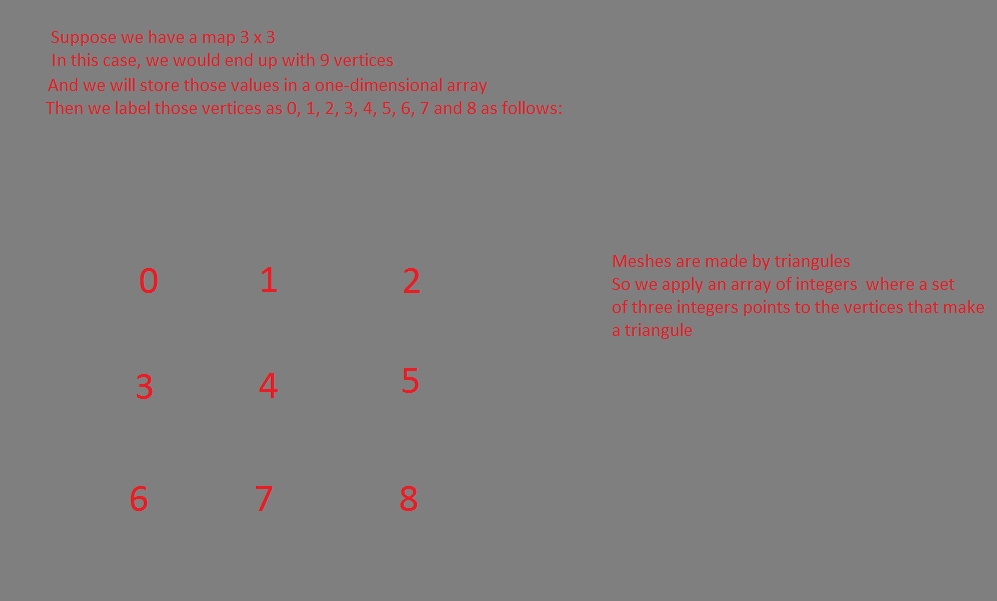
\includegraphics[height=80mm]{mesh_research_1.png}
\end{center}
\caption{Creating a map of 3x3 consist of 9 vertices}
\label{fig:pretty}
\end{figure}

\begin{figure}
\begin{center}
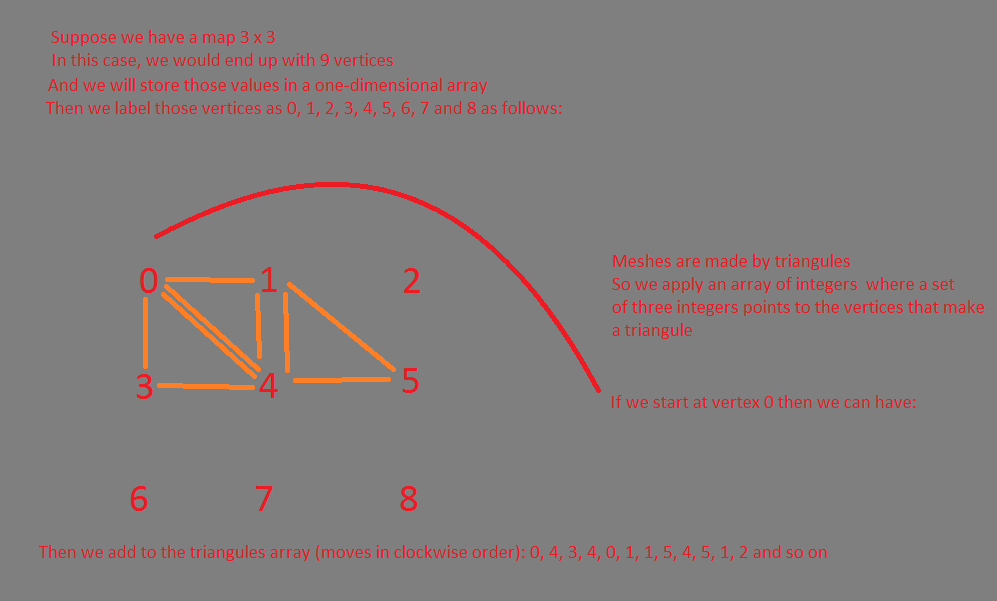
\includegraphics[height=80mm]{mesh_research_2.png}
\end{center}
\caption{Vertices are stored in a one-dimensional array and start at vertex 0}
\label{fig:pretty}
\end{figure}

\begin{figure}
\begin{center}
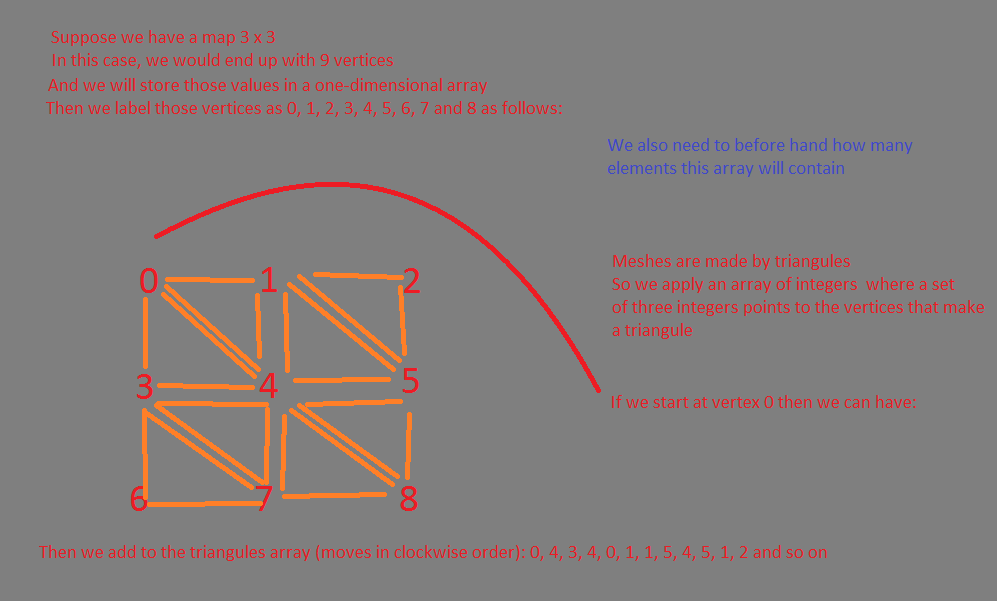
\includegraphics[height=80mm]{mesh_research_3.png}
\end{center}
\caption{All possible triangles in the map}
\label{fig:pretty}
\end{figure}


\begin{figure}
\begin{center}
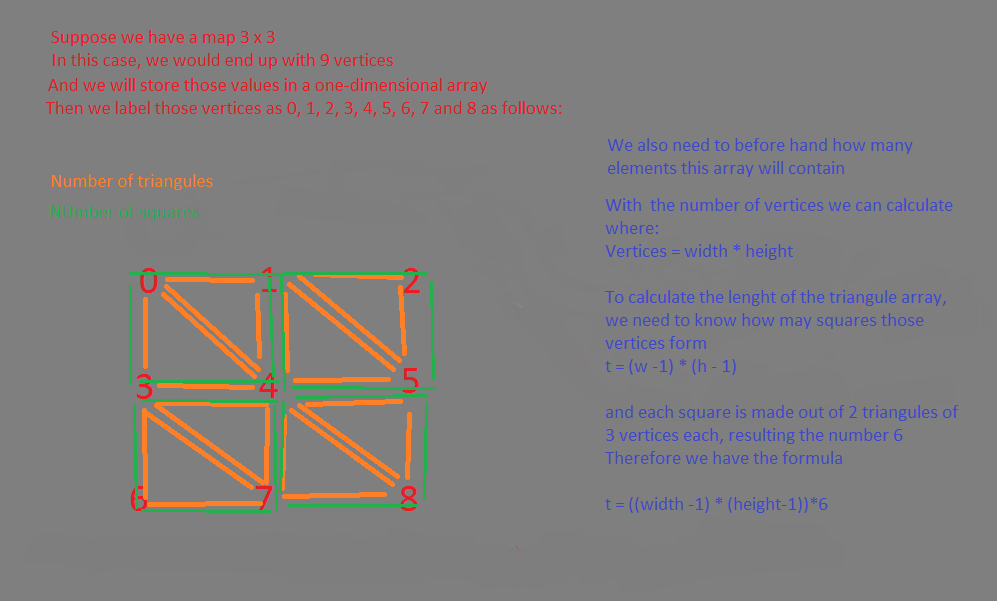
\includegraphics[height=80mm]{mesh_research_5.png}
\end{center}
\caption{Calculate the length of the triangle array}
\label{fig:pretty}
\end{figure}

\begin{figure}
\begin{center}
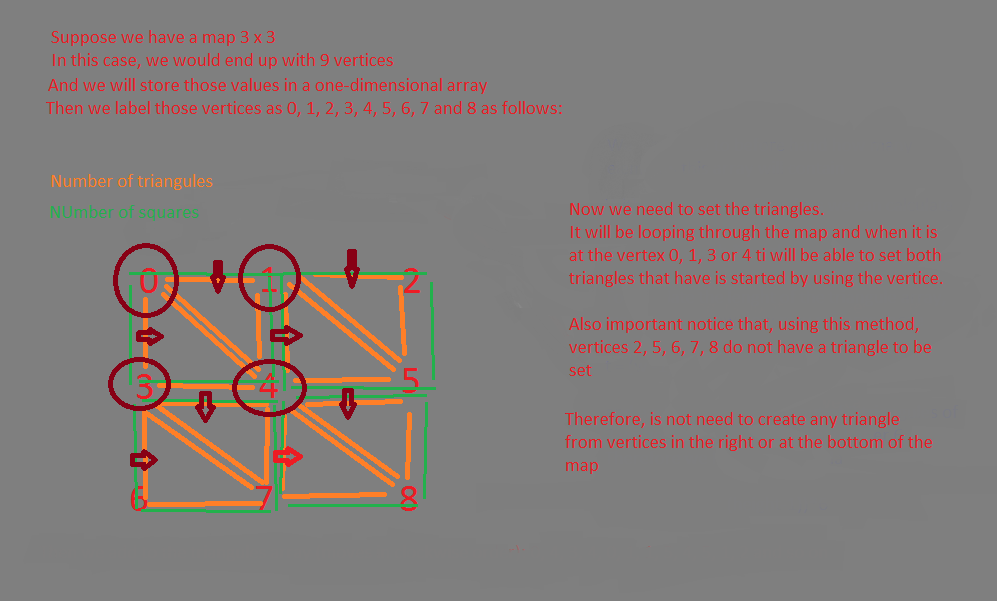
\includegraphics[height=80mm]{mesh_research_6.png}
\end{center}
\caption{What vertices can not create a triangule from the beginning}
\label{fig:pretty}
\end{figure}

\begin{figure}
\begin{center}
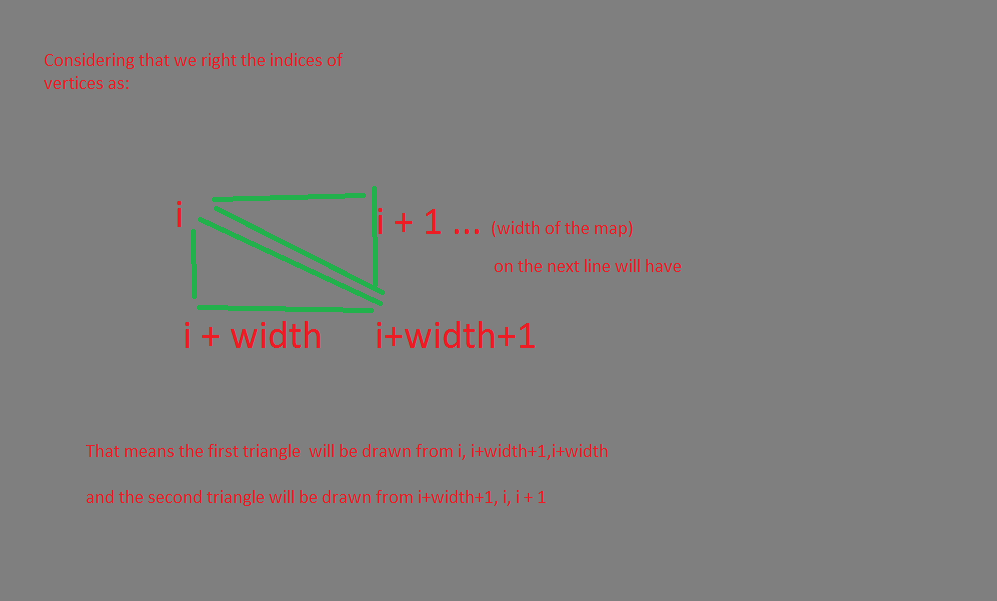
\includegraphics[height=80mm]{mesh_research_7.png}
\end{center}
\caption{Writing the vertices from 3x3 map to a one-dimension array}
\label{fig:pretty}
\end{figure}



\section{C-sharp steps}

1- The program need to generate a noise map, more specifically using perlin noise

2- Generate a two-dimensional array where the x and y grid coordinates are the indexes of the array

3- Store the noise values to the array

4- Generate a one-dimensional array colour map from a two-dimensional array height map

5- Generate textures to display noise map and colour map

5- Display the noise map and colour map on the scene

6- Add a new texture map to be added to the mesh

7- Create a mesh from the colour map, adapt it to re-scale the Y-axis

8-  Try to crash the program


\chapter{Implementation}
\label{chap:implementation}

In this chapter, the implementation of the project will be explained in detail. The code for the critical parts of the project will be included here with a correlated description of how the code works, what is doing and what result it achieves.
The chapter is broken down into sections in the same order of implementation when writing the code.


\section{C-sharp Programme in Unity3D Game Engine}

The following code is some of the key programming features of the project. It is written in the programme language -sharp, in Visual Studio for Unity3D game engine game engine. It is explained in detail. The complete code of the program will be added to the appendix.

The program is divided into 6 parts: 

1st part is the creation of a noise generator

2nd part is the creation of a map generator

3rd is the creation a map displayer

4th is the creation of an editor setting

5th is the creation of a texture generator

6th is the creation of a mesh generator


Disclaimer: in order to obtain more flexibility when writing and testing the code in Unity3D game engine, most of the variables DO NOT respect the encapsulation rule for object oriented programming. 

 
\subsection{Noise Generator}

The following code is the final version of the a NoiseGenerator class. It is one of the most important features of the entire program. It is responsible for create and store perlin values by using the build-in random perlin noise function: Mathf.PerlinNoise(float a, float b) to a two-dimensional array. It also made use of seed, and therefore one could repeat the same noise map once the parameters a set equal of a previous one.

It does not inherit from monobehaviour because it will not be instantiated any object from it in the scene and will also be a static class because it does not need to create multiple instances of this class.

\begin{lstlisting}
  
public static  class NoiseGenerator  {

    // a method to generate a noise map and return a grid o values to be returned between 0 and 1

    public static float [,] MapNoiseGenerator (int mapWidth, int mapHeight, 
        float scale, int numberOctaves, float persistance, float lacunarity, int seed, Vector2 offset)
    {
    
\end{lstlisting}

The class start with a function with a massive number of parameters. 
The MapNoisegenerator take as parameters 8 values: mapWidth and mapHeight are the dimensions of the terrain that will be created. numberOctaves are the number of layers, or number of noise maps that the terrain will have. Seed is an integer that controls the creation of pseudo random number generation. With the build-in system of Unity3D, when a parameter is entered, the random number will always be the same. If the seed is always the same, the ‘random number’ will always be the same.
Persistence is related to control the decrease of amplitude of the octaves and lacunarity is related to control the increase of frequency of the octaves.


\begin{lstlisting}
float[,] mapNoise = new float[mapWidth, mapHeight];

        System.Random pseudoRandomNumberGenerator = new System.Random(seed);
        // In order to sampling from different locations, and array of vector2 is used
        Vector2[] octaveOffsets = new Vector2[numberOctaves];


\end{lstlisting}

Then a two-dimensional array of float is used to store the map noise generated by the class and afterwards transfer the information to different parts of the code.
Then a pseudo random number generator is used to delivery numbers. A seed is passed as parameter to allow the reproduction of same noise maps.
To store samples from different parts of the noise map, a 2D vector is used and its size is the number of layers that the ultimate noise map will have, provided by the number of octaves.

\begin{lstlisting}

for(int i = 0; i < numberOctaves; i++)
        {

            // we also could scroll through the noise by providing our own offset value 
            float offsetX = pseudoRandomNumberGenerator.Next(-100000, 100000) + offset.x;
            float offsetY = pseudoRandomNumberGenerator.Next(-100000, 100000) + offset.y;

            octaveOffsets[i] = new Vector2(offsetX, offsetY);
        }

\end{lstlisting}
 
This for loop have a special intension. To iterate through the number of octaves or noise layers and generate two numbers in between a hundred thousand negative and a hundred thousand, plus a user input offset, for both x and y coordinates. It will then store the values into the Vector2D array. 

\begin{lstlisting}

// an error handler in case of scale is set to 0 (impossible division by zero)

        if (scale <= 0)
        {
            scale = 0.000001f;
        }

\end{lstlisting}

The next piece of code is simply an error handler to avoid the division by zero.


\begin{lstlisting}

for (int y = 0; y < mapHeight; y++)
        {
            for (int x = 0; x < mapWidth; x++)
            {

                float amplitude = 1;
                float frequency = 1;
                float noiseHeight = 0;

                for(int i = 0; i < numberOctaves; i++)
                {

                    // accessing sample coordinates
                    // adding a scale for the noise in order to not get rounded integer values
                    // the higher the frequency, more distant the sample points will be and therefore, more
                    // rapidly that values will change
                    float coordinateSampleX = (x - halfWidth) / scale * frequency + octaveOffsets[i].x;
                    float coordinateSampleY = (y - halfHeight) / scale * frequency + octaveOffsets[i].y; 
                    // generate a 2D perlin noise value
                    // by multiplying by 2 and subtracting by 1 we will
                    // increase the range from 0 to 1 to -1 to 1, since the PerlinNoise function only deliveries
                    // values in the range of 0 to 1
                    float perlinValue = Mathf.PerlinNoise(coordinateSampleX, coordinateSampleY) * 2 -1;
                    // apply the values to the noise map
                    noiseHeight += perlinValue * amplitude;

                    // at the end of each octave
                    amplitude *= persistance;
                    frequency *= lacunarity;
                }

                if(noiseHeight > maxNoiseValue)
                {
                    maxNoiseValue = noiseHeight;
                } else if(noiseHeight < minNoiseValue)
                {
                    minNoiseValue = noiseHeight;
                }
                // it will apply the noiseHeight to the noiseMap
                mapNoise[x, y] = noiseHeight;               
            }
        }

\end{lstlisting}

The code above is the heart of the noise generator class. It iterates the noise map two-dimensional array to store noise height values. It accesses a particular coordinate, within an octave (or layer). Then to calculate a noise value to a particular sample, it divides the coordinate sample by the scaler, multiply by the frequency, which a higher frequency, more distant the sample point will be and therefore more rapidly changes will occur and add on octave offset.
Then invoke the build-in perlin noise function of Unity3D game engine, which we already explain how it works during our research explanation of requirements. Calculates the perlin noise value to the coordinate sample for both x and y access. 

To make more interesting results, we enlarge the range of the perlin noise from the default mode from 0 to 1 to -1 to 1 by multiplying the perlin noise value by 2 and subtracting 1.

Apply persistance and lacunarity to amplitude and frequency respectively. 
In order to be able to normalized afterwards, the maximum and minimum noise values are saved.
Finally, the function will return the noise map generated.


\subsection{Map Generator}

The map generator class must inherit from monobehaviour because will be instantiated in the scene. Once again a disclaimer here: all variables here DO NOT respect the encapsulation rule of the object oriented programming and are set to be public in order to easily changes in the inspector and instant feedback.

\begin{lstlisting}

public class MapGenerator : MonoBehaviour {

    // Create a enumerator to determine which mode it will be displayed
    public enum DisplayMode { NoiseMap, ColourMap, Mesh};
    public DisplayMode displayMode;

    public int mapWidth;
    public int mapHeight;
    public float scale;
    public int numberOfOctaves;
    [Range(0, 1)] // set the persistance to range between 0 and 1
    public float persistance;
    public float lacunarity;
    public int seed;
    public Vector2 offset;
    // a boolean to update the noise map when the generateMap is pressed again
    public bool updateNoiseMap;
    public TypesOfTerrain[] biomes;
    public float meshHeightValueMultiplier;
    public AnimationCurve meshHeightCurve; 
    

\end{lstlisting}

Almost all input that can be changed by the user is found here. Variables are defined here first, such as octaves, persistence and lacunarity, seed, and is carried out through the program from here.

The first thing in the class is to declare an enumeration of three different types of enumerators, which are one for noise map mode, another one for colour map mode and finally one to display a mesh mode. Also creates a reference to an DisplayMode object called displayMode.

The range of the persistence is set be in between 0 and 1. Later in the code, other constrains to those variables are added.

Also a reference to a struct array is created. This struct will hold all the possible biomes that someone can enter in the inspector.

A float that will store the value that will actually multiplier the Y-axis of the 3D mesh making all the terrain goes up from its original point.
Last variable is an animation curve to deal with the problem encountered when there is not a trash-hold for the height value of the water biome.

\begin{lstlisting}

public void mapGen()
    {
        float[,] noiseMap = NoiseGenerator.MapNoiseGenerator(mapWidth, mapHeight, scale, numberOfOctaves, persistance, lacunarity, seed, offset);
        Color[] colourMap = new Color[mapWidth * mapHeight];
        for(int y = 0; y < mapHeight; y++)
        {
            for (int x = 0; x < mapWidth; x++)
            {
                float currentHeightValue = noiseMap[x, y];
                for(int j = 0; j < biomes.Length; j++)
                {
                    if(currentHeightValue <= biomes[j].height)
                    {
                        colourMap[y * mapWidth + x] = biomes[j].colour;
                        break; // we have found our biome and dont need to continue
                    }
                } 
            }
        }
        // Reference to map displayer class
        MapDisplayer dis = FindObjectOfType<MapDisplayer>();
        if(displayMode == DisplayMode.NoiseMap)
        {
            dis.DrawTextureToScreen(TextureGenerator.TextureFromHeightMap(noiseMap));
        }
        else if(displayMode == DisplayMode.ColourMap)
        {
            dis.DrawTextureToScreen(TextureGenerator.TextureFromColourMap(colourMap, mapWidth, mapHeight));
        }
        else if(displayMode == DisplayMode.Mesh)
        {
            dis.DrawMeshToScreen(MeshCreator.TerrainMeshCreator(noiseMap, meshHeightValueMultiplier, meshHeightCurve), 
                                                TextureGenerator.TextureFromColourMap(colourMap, mapWidth, mapHeight));
        }
        
    }

\end{lstlisting}

The mapGen function is responsible for actually generate the colour map from the noise map.

It will iterate through the values of the noise map, and based on the values of each biome, which were set in the inspector, will store a colour value to an array of colours for that particular x and y coordinate.
The function will also check which mode is currently set in the inspector, and then will call the display function of the appropriated mode to be drawn in the scene.

\begin{lstlisting}

void OnValidate()
    {
        if(mapWidth < 10)
        {
            mapWidth = 10;
        }
        if(mapHeight < 10)
        {
            mapHeight = 10;
        }
        if (lacunarity < 1)
        {
            lacunarity = 1;
        }
        if (numberOfOctaves < 1)
        {
            numberOfOctaves = 1;
        }
    }

\end{lstlisting}

This function just imposes limits to the values, acting like constrains of values in the inspector.


\subsection{Map Displayer}

This class is a support class for this project.
Using many build-in features of Unity3D game engine, such as, the Renderer class, MeshFilter class, MeshRenderer class and Texture2D. It allows the display of the textures and meshes on the screen.

It set a reference to the plane primitive game object in the scene, so then we could manipulate values on it and render textures, attached to materials using shaders, by using the textureRenderer renderer to transform a 2D texture in a 3D world space. This is exact what happen when textureRenderer.transform.localScale = new Vector3(texture.width, 1, texture.height); is invoked. 

// It will also be instantiate in the scene and therefore must inherit from monobehaviour

\begin{lstlisting}

public class MapDisplayer : MonoBehaviour {

    // Here we will need to set a reference of the renderer of the plane in the scene to be used
    // later on the set its texture

    public Renderer textureRenderer;
    // a public reference to a mesh filter
    public MeshFilter meshFilter;
    // a public reference to a mesh renderer
    public MeshRenderer meshRenderer;

    public void DrawTextureToScreen(Texture2D texture)
    {
        textureRenderer.sharedMaterial.mainTexture = texture;
        textureRenderer.transform.localScale = new Vector3(texture.width, 1, texture.height);
    }

    public void DrawMeshToScreen(MeshData meshData, Texture2D texture)
    {
        meshFilter.sharedMesh = meshData.CreateMesh();
        meshRenderer.sharedMaterial.mainTexture = texture;
    }
}

\end{lstlisting}

\subsection{Editor Setting}

The editor setting class as works for monobehaviour, inherits its functionalities from the UnityEditor library, and therefore it inherits from the Editor super class.

In the editor setting class a public void function that allow this class to override OnInspectorGUI UnityEditor function is created.

\begin{lstlisting}

public override void OnInspectorGUI()

\end{lstlisting}


This function is needed to create a reference to the map generator class.


\begin{lstlisting}

MapGenerator mg = (MapGenerator)target;

Where the word target here is the object that this custom editor is inspecting and then cast that object to a map generator.

if (DrawDefaultInspector())
{
     if (mg.updateNoiseMap)
     {
           mg.mapGen();
     }
}

if(GUILayout.Button("GenerateMap"))
{
     mg.mapGen();
}

\end{lstlisting}

The first of the nested if statement is to detected when the default inspector, and in the second nested if statement, the object mg, in case of its updateNoiseMap box is selected, it will generate a map.
The second if statement creates a button writing now on it GenerateMap. Once this button is pressed, it will also generate the map. 


\subsection{Texture Generator}

The texture generator class is a class used to generate textures within two different possibilities, from a height map and from a colour map.

Due to the fact that this class will not be instantiated in the scene, it will not inherit from monobehaviour. It will also be a static void once we do not need multiple instances of this class.

\begin{lstlisting}

// This will create a texture from an one-dimensional array colour map
    public static Texture2D TextureFromColourMap(Color [] colourMap, int width, int height)
    {
        Texture2D texture = new Texture2D (width, height);
        // This fix the blurring effect of the texture
        texture.filterMode = FilterMode.Point; // instead of bilinear
        // To fix the border of the map
        texture.wrapMode = TextureWrapMode.Clamp;
        texture.SetPixels(colourMap);
        texture.Apply();
        return texture;
    }

\end{lstlisting}

The first function of this class is to generate a texture from a colour map stored in an one-dimensional array of colours, as the name suggests TextureFromColourMap.
It takes 3 parameters, one being the already mentioned one-dimensional array of colours, a width and a height for that colour.

Then a reference to an 2D texture in Unity3D is created using the parsed width and height.

The next two lines of code is just to correct some of the blurring and wrap imperfections of the map created.

Then we set to the texture the values in the colour map itself. Then finally we apply the buffered texture to the texture variable itself and return it.


\begin{lstlisting}

// another method to get a texture based on a 2D height map
    public static Texture2D TextureFromHeightMap(float[,] heightMap)
    {
        int width = heightMap.GetLength(0); // for the first dimension
        int height = heightMap.GetLength(1); // for the second dimension

        // Create a colour array to store all the colour of the pixels.
        // For efficiency, all values will be added to a one-dimensional array
        Color[] colourMapContainer = new Color[width * height];

        //Then I need to loop through noiseMap array to extract the value
        for (int y = 0; y < height; y++)
        {
            for (int x = 0; x < width; x++)
            {
                // This technique is used to turn values from a two-dimensional array
                // into a one-dimensional array
                // in the lerp function, the first 2 parameters are the colours set as minimum and
                // maximum values to lerp through, and the percentage will be 0 and 1, which is the same
                // as the range of the noiseMap
                colourMapContainer[y * width + x] = Color.Lerp(Color.black, Color.white, heightMap[x, y]);
            }
        }
        return TextureFromColourMap (colourMapContainer, width, height);
    }

\end{lstlisting}

This second function of the class texture generator is used to return a 2D texture from a two-dimensional array height map.

The first two variables in the body of this function width and height and both are checked by the size of the two-dimensional array, where 0 is the marking the beginning and 1 is the end of the array.

Then a one-dimensional array of type Color is instantiated to store all the colour values of the pixels.

A nested for loop to iterate through the two-dimensional array to extract the values in it and store them into the one-dimensional array. Before those values are stored, a Lerp function from the Color class is used to interpolate the values of the height map into a black and white gradient. Where black is the minimum value of 0, white is the maximum value of 1, and all other values in the height map are interpolated within this range of 0 and 1.


\subsection{Mesh Creator}

Mesh creator class is another key feature of this program. It generates a flat plane setting the height of individual vertices, creates the terrain mesh for this project.

It is a static class and do not extend from monobehaviour class.
The only function of the class returns a Mesh Data object and it is called TerrainMeshCreator.

First two variables sets of variables declare and initialize the width and height that is used as parameters of the reference of a MeshData class variable called meshData.  The last variable is the vertexIndex and its goal it to keep track of the index in the triangules array in the meshData object.

The nested for loop is used to iterate in the two-dimensional array heightMap and inside of its body set the vertices array in the meshData current object to be the values of the topLeftX coordinate of the triangle in the X-axis, in the Y-axis a threshold that uses the build-in function Evaluate(), which as the names suggests, evaluate the a value. In this case, the value is the height value in the heightMap multiplied by a modifier called heightValueMultiplier. And for last, the Z-axis is filled with the value of the topLeftZ subtract by Y coordinate.

To the mesh be perfectly centred on the screen, we have considered three points: 

x, x, x

In order to this to be centred, the x value must have the value of zero, the one on the left must have value -1 and to the right value equal to 1.
We can work out the value of the most x left point by going to x = ((width -1)/-2). In this case, width is the number of points, which is three. X = 3-1/-2 = -1

For this reason, we have declared and initialized the variables topLeftX and topLeftZ with the respective values.

\begin{figure}
\begin{center}
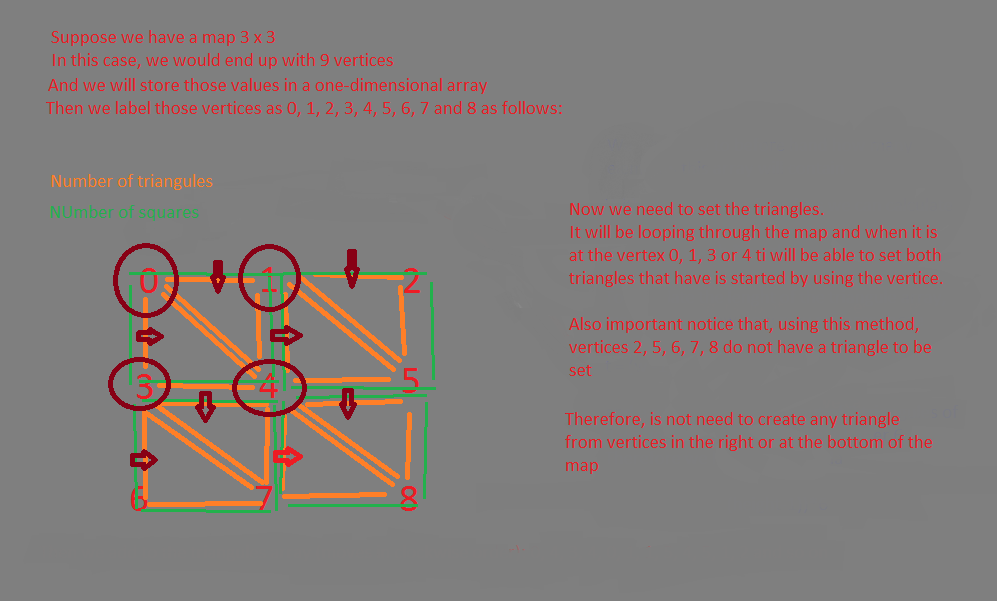
\includegraphics[height=70mm]{mesh_research_6.png}
\end{center}
\caption{Recapitulation of how the triangles are formed in the program}
\label{fig:pretty}
\end{figure}
 

In the if statement (x < width – 1 and y < height -1) we are simply ignoring the right and bottom values of the map as shown in the figure above. Then we can add the two triangles that the square is made of, by following the rule in the chart Figure 4.2:

\begin{figure}
\begin{center}
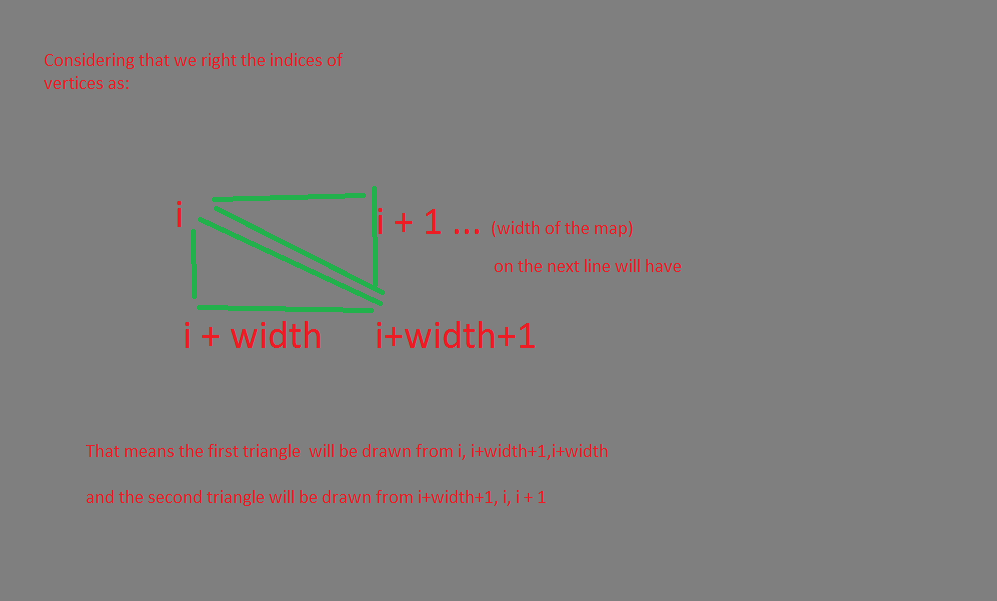
\includegraphics[height=70mm]{mesh_research_7.png}
\end{center}
\caption{Recapitulation of how the triangles are formed in the program}
\label{fig:pretty}
\end{figure}
 
\begin{lstlisting}
 
public static MeshData TerrainMeshCreator(float [,] heightMap, float heightValueMultiplier, AnimationCurve trashHold)
    {
        int width = heightMap.GetLength(0);
        int height = heightMap.GetLength(1);
        float topLeftX = (width - 1) / -2f;
        float topLeftZ = (height - 1) / 2f;
        MeshData meshData = new MeshData(width, height);
        int vertexIndex = 0;

        // Need a loop to go through the heightMap
        for(int y = 0; y < height; y++)
        {
            for(int x = 0; x < width; x++)
            {
                meshData.vertices[vertexIndex] = new Vector3(topLeftX + x, trashHold.Evaluate(heightMap[x, y]) * heightValueMultiplier, topLeftZ - y);
                meshData.uvs[vertexIndex] = new Vector2(x / (float)width, y / (float)height);

                if(x < width -1 && y < height - 1)
                {
                    meshData.AddTriangule(vertexIndex, vertexIndex + width + 1, vertexIndex + width);
                    meshData.AddTriangule(vertexIndex + width + 1, vertexIndex, vertexIndex + 1);
                }
                vertexIndex++;
            }
        }
        return meshData;
    }
\end{lstlisting}


\subsection{Mesh Data}

This class stores most of the data-structure to create the mesh of the program, with exception of the noise values.

It declares a vector3 array of vertices, to store obviously, the vertices of a given triangle. It also declares a variable to store the triangles in an integer array and a vector2 array to store the UV, also known as texture coordinates (to differentiate of the XYZ world coordinates).

A quick explanation about UV map extract from the online source http://blenderartists.org/forum/archive/index.php/t-173777.html last visited on 16/08/2016.

"The UV map contains a polygon (which, by definition, is "flat") for every face (which is also "flat") of the object.

The location of the face, on the object, is expressed using (X, Y, Z) coordinates.

The location of the polygon, on the image, is (U, V, [W]).

So, to find what to draw onto any face, the computer consults the UV map. The polygon on the map, which corresponds to the face on the object, provides the location of the image-data that should be used."

Then its constructor will initialize the declared variables mentioned above following the rules of Figure 4.3:
 
\begin{figure}
\begin{center}
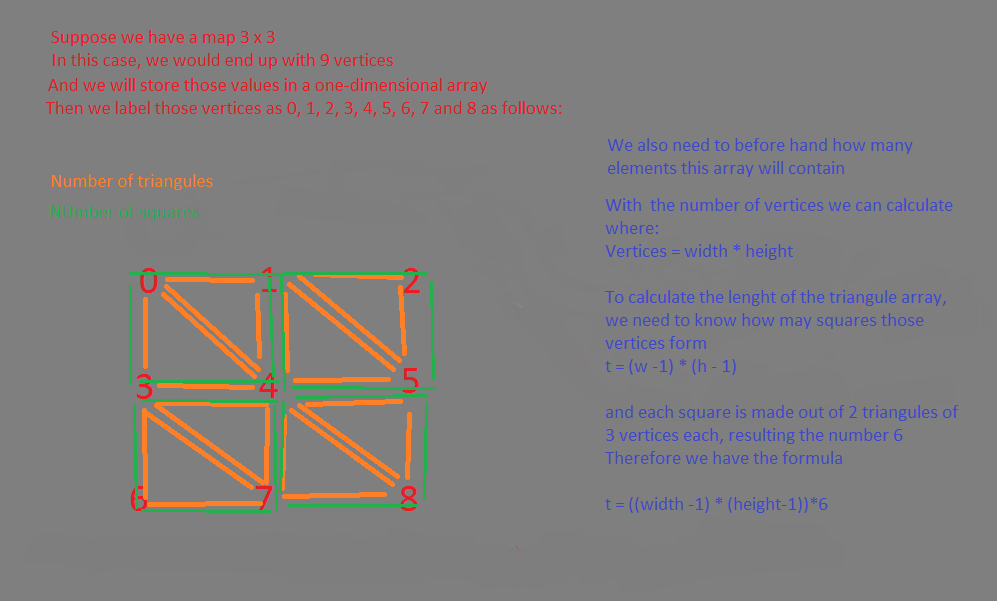
\includegraphics[height=70mm]{mesh_research_5.png}
\end{center}
\caption{Recapitulation of how the triangles are formed in the program}
\label{fig:pretty}
\end{figure}

Where the size of the array of vertices is given by the formula vertices = width * height, same for the UV and the size of the triangles array is calculated by the formula: 

(width – 1) * (height-1) * 6.



\begin{lstlisting}

public Vector3[] vertices;
    public int[] triangules;
    // UV map to create textures in 2D to be applied to a 3D object
    public Vector2[] uvs;

    // to keep track of the current trianguloe index
    int trianguleIndex;

    public MeshData(int meshWidth, int meshHeight)
    {
        vertices = new Vector3[meshWidth * meshHeight];
        //We need here an UV for each vertex
        uvs = new Vector2[meshWidth * meshHeight];
        // we need to know where it is each vertex in relation to the rest of the map
        // as percentage of both x and y axis
        // this percentage would be between 0 and 1
        triangules = new int[(meshWidth - 1) * (meshHeight - 1) * 6];
    }


\end{lstlisting}


The second part of the class is a function take three vertices and add then to form a triangle and then incrementing a variable that keeps track of the triangle index array.


\begin{lstlisting}


public void AddTriangule (int firstVertice, int secondVertice, int thirdVertice)
    {
        triangules[trianguleIndex] = firstVertice;
        triangules[trianguleIndex + 1] = secondVertice;
        triangules[trianguleIndex + 2] = thirdVertice;

        // increment the triangule index
        trianguleIndex += 3;
    }


\end{lstlisting}

In the last part of the class a create mesh function that returns a mesh object to its caller.
First it creates a reference to a mesh game object in Unity3D. Then it assigns the values of the vertices, triangles and UVs to a particular object at the time, use a build-in function in Unity3D to recalculate the normal for lighting and finally return the mesh.


\begin{lstlisting}


public Mesh CreateMesh()
    {
        Mesh mesh = new Mesh();
        mesh.vertices = vertices;
        mesh.triangles = triangules;
        mesh.uv = uvs;
        mesh.RecalculateNormals(); // In order to light work properly
        return mesh;
    }

\end{lstlisting}

\chapter{System Testing and Evaluation}
\section{How my system/software can be tested}

The system can tested not during run time, can me instantly tested by twinkling values in the direct in the inspector and get the immediate feedback at the scene view window of Unity3D game engine.

There is three different possible checks in the system.

1- check the generation of the noise map

2- check the generation of the colour map

3- check the generation of the mesh based on the colour map

The system allow to reproduce a previous map generated by using a seed




\section{The results of testing my system/software}

Some constrains were added to make the system more stable and error handler added in one case to avoid division by zero.

Some of these constrains can be observed in the Map Generator class, within the void method OnValidate().

The system perform pretty consistent to produce noise maps and colour maps.

There is still issues to be solved related to the mesh generator. Although the code runs pretty well during the first time the mesh is generated, I could not manage in time to reset the mesh when another view mode is selected, such noise mode or colour mode.

\section{How I might improve my project based on this evaluation}

The project could greatly improve by adding more features to it, such as, dividing the map into chunks and then using already implemented offset parameters, make the generation of an infinite terrain generation.

Also, the project could be improved my fixing the reset problem of the mesh generator after run for the first time.

Another option could be the implementation of more details textures for each biome of the system.

\chapter{Summary and Conclusions}
\section{System Success}

The system successfully implement both noise and colour maps with good efficiency. Overall, evaluation is that most of the goals added to the first project proposal were implemented. The map generated by the code are very flexible to change, highly customizable by the user, which following the definition of Procedural Content Generation, have indirect input on the system.

The system also creates mesh from a generated colour map instead of using the Unity Terrain Package and just deform the Y-axis parameter, which I consider a personal achievement. 

\section{System Failure}

The system still have some issues related to the mesh generator after being used for the first time and have not been fixed. The most obvious failure for this project was the proposal of the code to generate infinite chunks of terrain and due time and complexity constrains, was not possible to be implement.

\section{Project Self-Evaluation}

I am happy that I have finally accomplish this last assignment for my degree, feeling of job done, specially taking into account the turmoil that my personal life presented during the last 8 months.

In terms of freedom of work and decision making process, which was the very first project done completely by myself, it was a bit strange. Students could have more opportunities to work alone if so desired.

In terms of learning this project allowed me to explore in more depth two modules of my degree which I have enjoy very much to study. Graphics and the mathematical formula to represent objects in a computer screen (to create textures and meshes) and random number generators, that are actually pseudo-random.



\part{appendix}
\chapter{C-sharp Program}


 The Noise Generator Class
 
\begin{lstlisting}
using UnityEngine;
using System.Collections;

// It will be static because it does not need to create multiple instances of this class
// dont need to inherit from monobehaviour because it will not be applied to any object in the scene


    
public static class NoiseGenerator  {

    // a method to generate a noise map and return a grid o values to be returned between 0 and 1

    public static float [,] MapNoiseGenerator (int mapWidth, int mapHeight, 
        float scale, int numberOctaves, float persistance, float lacunarity, int seed, Vector2 offset)
    {
        float[,] mapNoise = new float[mapWidth, mapHeight];

        System.Random pseudoRandomNumberGenerator = new System.Random(seed);
        // In order to sampling from different locations, and array of vector2 is used
        Vector2[] octaveOffsets = new Vector2[numberOctaves];
        for(int i = 0; i < numberOctaves; i++)
        {

            // we also could scroll through the noise by provading our own offset value 
            float offsetX = pseudoRandomNumberGenerator.Next(-100000, 100000) + offset.x;
            float offsetY = pseudoRandomNumberGenerator.Next(-100000, 100000) + offset.y;

            octaveOffsets[i] = new Vector2(offsetX, offsetY);
        }

        // an error handler in case of scale is set to 0 (impossible division by zero)

        if(scale <= 0)
        {
            scale = 0.000001f;
        }

        float maxNoiseValue = float.MinValue; // float is set to the minimum possible value
        float minNoiseValue = float.MaxValue; // same as above but set to the maximum value

        // when we scale the mapNoise, the values are calculated from the top right corner
        // to fix this problem we calculate the half width and half height and apply those 
        // values to coordinateSample x and y
        float halfWidth = mapWidth / 2f;
        float halfHeight = mapHeight / 2f;

        // nested for loop to iterate within the bi-dimmensional array
        for (int y = 0; y < mapHeight; y++)
        {
            for (int x = 0; x < mapWidth; x++)
            {

                float amplitude = 1;
                float frequency = 1;
                float noiseHeight = 0;

                for(int i = 0; i < numberOctaves; i++)
                {

                    // accessing sample coordinates
                    // adding a scale for the noise in order to not get rounded interger values
                    // the higher the frequency, more distant the sample points will be and therefore, more
                    // rapidly tha values will change
                    float coordinateSampleX = (x - halfWidth) / scale * frequency + octaveOffsets[i].x;
                    float coordinateSampleY = (y - halfHeight) / scale * frequency + octaveOffsets[i].y; 
                    // generate a 2D perlin noise value
                    // by multipling by 2 and subtracting by 1 we will
                    // inscrease the range from 0 to 1 to -1 to 1, since the PerlinNoise function only deliveries
                    // values in the range of 0 to 1
                    float perlinValue = Mathf.PerlinNoise(coordinateSampleX, coordinateSampleY) * 2 -1;
                    // apply the values to the noise map
                    noiseHeight += perlinValue * amplitude;

                    // at the end of each octave
                    amplitude *= persistance;
                    frequency *= lacunarity;
                }

                if(noiseHeight > maxNoiseValue)
                {
                    maxNoiseValue = noiseHeight;
                } else if(noiseHeight < minNoiseValue)
                {
                    minNoiseValue = noiseHeight;
                }
                // it will apply the noiseHeight to the noiseMap
                mapNoise[x, y] = noiseHeight;               
            }
        }

        // Now, we need to normalize the values to get back again values from 0 to 1
        // to do that, we need to keep track of the minimum and maxium values
        for (int y = 0; y < mapHeight; y++)
        {
            for (int x = 0; x < mapWidth; x++)
            {
                // the inverse lerp method returns a value between 0 and 1
                // where the same value of minNoiseValue will return zero and
                // same value of maxNoiseValue will return 1
                mapNoise[x, y] = Mathf.InverseLerp(minNoiseValue, maxNoiseValue, mapNoise[x, y]);
            }
        }

        return mapNoise;
    }
}

\end{lstlisting}

The Map Generator Class

\begin{lstlisting}
using UnityEngine;
using System.Collections;

// This script will be instantiate in the scene by unity and therefore needs
// to inherit from monobehaviour class
public class MapGenerator : MonoBehaviour {

    // Create a enumerator to determine which mode it will be displayed
    public enum DisplayMode { NoiseMap, ColourMap, Mesh};
    public DisplayMode displayMode;

    public int mapWidth;
    public int mapHeight;
    public float scale;
    public int numberOfOctaves;
    [Range(0, 1)] // set the persistance to range between 0 and 1
    public float persistance;
    public float lacunarity;
    public int seed;
    public Vector2 offset;
    // a boolean to update the noise map when the generateMap is pressed again
    public bool updateNoiseMap;
    public TypesOfTerrain[] biomes;
    public float meshHeightValueMultiplier;
    public AnimationCurve meshHeightCurve;

    public void mapGen()
    {
        float[,] noiseMap = NoiseGenerator.MapNoiseGenerator(mapWidth, mapHeight, scale, numberOfOctaves, 
                                                             persistance, lacunarity, seed, offset);
        Color[] colourMap = new Color[mapWidth * mapHeight];
        for(int y = 0; y < mapHeight; y++)
        {
            for (int x = 0; x < mapWidth; x++)
            {
                float currentHeightValue = noiseMap[x, y];
                for(int j = 0; j < biomes.Length; j++)
                {
                    if(currentHeightValue <= biomes[j].height)
                    {
                        colourMap[y * mapWidth + x] = biomes[j].colour;
                        break; // we have found our biome and dont need to continue
                    }
                } 
            }
        }
        // Reference to map displayer class
        MapDisplayer dis = FindObjectOfType<MapDisplayer>();
        if(displayMode == DisplayMode.NoiseMap)
        {
            dis.DrawTextureToScreen(TextureGenerator.TextureFromHeightMap(noiseMap));
        }
        else if(displayMode == DisplayMode.ColourMap)
        {
            dis.DrawTextureToScreen(TextureGenerator.TextureFromColourMap(colourMap, mapWidth, mapHeight));
        }
        else if(displayMode == DisplayMode.Mesh)
        {
            dis.DrawMeshToScreen(MeshCreator.TerrainMeshCreator(noiseMap, meshHeightValueMultiplier, meshHeightCurve), 
                                                TextureGenerator.TextureFromColourMap(colourMap, mapWidth, mapHeight));
        }
        
    }

    // To impose limits to the values in the inspector, we can camp some of the values
    // to be in a certain range
    // The function OnValidate is called automatically whenever one variable is changed in the inspector

    void OnValidate()
    {
        if(mapWidth < 10)
        {
            mapWidth = 10;
        }
        if(mapHeight < 10)
        {
            mapHeight = 10;
        }
        if (lacunarity < 1)
        {
            lacunarity = 1;
        }
        if (numberOfOctaves < 1)
        {
            numberOfOctaves = 1;
        }
    }	
}

[System.Serializable] // to be seem in the inspector
public struct TypesOfTerrain
{
    public string nameOfBiome;
    public float height;
    public Color colour;
}

\end{lstlisting}

The Map Displayer Class

\begin{lstlisting}
using UnityEngine;
using System.Collections;

// It will also be intantiate in the scene and therefore must inherit from monobehaviour
public class MapDisplayer : MonoBehaviour {

    // Here we will need to set a reference of the renderer of the plane in the scene to be used
    // later on the set its texture

    public Renderer textureRenderer;
    // a public reference to a mesh filter
    public MeshFilter meshFilter;
    // a public reference to a mesh renderer
    public MeshRenderer meshRenderer;

    public void DrawTextureToScreen(Texture2D texture)
    {
        textureRenderer.sharedMaterial.mainTexture = texture;
        textureRenderer.transform.localScale = new Vector3(texture.width, 1, texture.height);
    }

    public void DrawMeshToScreen(MeshData meshData, Texture2D texture)
    {
        meshFilter.sharedMesh = meshData.CreateMesh();
        meshRenderer.sharedMaterial.mainTexture = texture;
    }
}

\end{lstlisting}

The Editor Settings Class

\begin{lstlisting}
using UnityEngine;
using System.Collections;
using UnityEditor;

// Will inherit from editor class
[CustomEditor (typeof (MapGenerator))]

public class EditorSettings : Editor {

    public override void OnInspectorGUI()
    {
        // We need here a reference to the Map Generator class
        // target here is object that this custom editor is inspecting 
        // and cast that object to a map generator
        MapGenerator mg = (MapGenerator)target;

        if (DrawDefaultInspector())
        {
            if (mg.updateNoiseMap)
            {
                mg.mapGen();
            }
        }

        if(GUILayout.Button("GenerateMap"))
        {
            mg.mapGen();
        }
    }
}

\end{lstlisting}

The Texture Generator Class

\begin{lstlisting}
using UnityEngine;
using System.Collections;

public static class TextureGenerator {

    // This will create a texture from an one-dimensional array colour map
    public static Texture2D TextureFromColourMap(Color [] colourMap, int width, int height)
    {
        Texture2D texture = new Texture2D(width, height);
        // This fix the bluring effect of the texture
        texture.filterMode = FilterMode.Point; // instead of bilinear
        // To fix the border of the map
        texture.wrapMode = TextureWrapMode.Clamp;
        texture.SetPixels(colourMap);
        texture.Apply();
        return texture;
    }

    // another method to get an texture based on a 2D height map
    public static Texture2D TextureFromHeightMap(float[,] heightMap)
    {
        int width = heightMap.GetLength(0); // for the first dimension
        int height = heightMap.GetLength(1); // for the second dimension

        // Create a colour array to store all the colour of the pixels.
        // For eficiency, all values will be added to an one-dimensional array
        Color[] colourMapContainer = new Color[width * height];

        //Then I need to loop through noiseMap array to extrat the value
        for (int y = 0; y < height; y++)
        {
            for (int x = 0; x < width; x++)
            {
                // This technique is used to turn values from a two-dimensional array
                // into an one-dimensional array
                // in the lerp function, the first 2 parameters are the colours set as minimum and
                // maximum values to lerp through, and the percentage will be 0 and 1, which is the same
                // as the range of the noiseMap
                colourMapContainer[y * width + x] = Color.Lerp(Color.black, Color.white, heightMap[x, y]);
            }
        }
        return TextureFromColourMap (colourMapContainer, width, height);
    }
}

\end{lstlisting}

The Mesh Creator Class

\begin{lstlisting}
using UnityEngine;
using System.Collections;

public static class MeshCreator {
    
    public static MeshData TerrainMeshCreator(float [,] heightMap, float heightValueMultiplier, AnimationCurve trashHold)
    {
        int width = heightMap.GetLength(0);
        int height = heightMap.GetLength(1);
        float topLeftX = (width - 1) / -2f;
        float topLeftZ = (height - 1) / 2f;
        MeshData meshData = new MeshData(width, height);
        int vertexIndex = 0;

        // Need a loop to go through the heightMap
        for(int y = 0; y < height; y++)
        {
            for(int x = 0; x < width; x++)
            {
                meshData.vertices[vertexIndex] = new Vector3(topLeftX + x, trashHold.Evaluate(heightMap[x, y]) * heightValueMultiplier, topLeftZ - y);
                meshData.uvs[vertexIndex] = new Vector2(x / (float)width, y / (float)height);

                if(x < width -1 && y < height - 1)
                {
                    meshData.AddTriangule(vertexIndex, vertexIndex + width + 1, vertexIndex + width);
                    meshData.AddTriangule(vertexIndex + width + 1, vertexIndex, vertexIndex + 1);
                }
                vertexIndex++;
            }
        }
        return meshData;
    }
}
\end{lstlisting}

The Mesh Data Class

\begin{lstlisting}
public class MeshData
{
    public Vector3[] vertices;
    public int[] triangules;
    // UV map to create textures in 2D to be applied to a 3D object
    public Vector2[] uvs;

    // to keep track of the current trianguloe index
    int trianguleIndex;

    public MeshData(int meshWidth, int meshHeight)
    {
        vertices = new Vector3[meshWidth * meshHeight];
        //We need here an UV for each vertex
        uvs = new Vector2[meshWidth * meshHeight];
        // we need to know where it is each vertex in relation to the rest of the map
        // as percentage of both x and y axis
        // this percentage would be between 0 and 1
        triangules = new int[(meshWidth - 1) * (meshHeight - 1) * 6];
    }

    public void AddTriangule (int firstVertice, int secondVertice, int thirdVertice)
    {
        triangules[trianguleIndex] = firstVertice;
        triangules[trianguleIndex + 1] = secondVertice;
        triangules[trianguleIndex + 2] = thirdVertice;

        // increment the triangule index
        trianguleIndex += 3;
    }

    public Mesh CreateMesh()
    {
        Mesh mesh = new Mesh();
        mesh.vertices = vertices;
        mesh.triangles = triangules;
        mesh.uv = uvs;
        mesh.RecalculateNormals(); // In order to light work properly
        return mesh;
    }
}
\end{lstlisting}


\bibliographystyle{apalike}
\bibliography{}
Bibliograph\\


Author Togelius, J., Author Kastbjerg, E., Author Schedl, D., AuthorYannakakis. (2011) title of the paper.What is procedural content generation?: Mario on the borderline. In: Proceedings of the 2nd Workshop on Procedural Content Generation in Games. website   http://julian.togelius.com/Togelius2011What.pdf ; last accessed 23/08/2016 \\

Author Shiffman, Daniel. (2012). Title of the paper. The Nature of Code: Simulating natural systems with processing \\

Author Van Verth, James M., Author Bishop, Lars M. (2004). Title of the paper. Essential Mathematics for Games: and interactive applications, chapters 4, 5 and 6.\\

Author Shakern, Noor., Tagelius, Julian., Nelson, Mark J. Title of the paper. Procedural Content Generation in Games. Website http://pcgbook.com/ ; last accessed: 23/08/2016.\\

Author Game Dev Blog. (2015) Title of the paper. Infinite terrain generation in Unity3D - part 1. Website http://code-phi.com/infinite-terrain-generation-in-unity-3d/ ; last visited on 23/08/216\\





\end{document}  
